\documentclass[]{report}
\usepackage{graphicx, float,}
\usepackage{hyperref}
\usepackage[export]{adjustbox}

\title{\centering CSP334 : Computer Networks \\Lab Assignment No 4\\Assignment on HTTP}
\author{\LARGE Sahil\\2016UCS0008}

% to use proper section numbering in the report type 
\renewcommand{\thesection}{\arabic{section}}

\begin{document} 

\maketitle

%%%%%%%%%%%%%%%%%%%%%%%%%%%%%%%%%%%%%%%%%%%%%%%%
\section{The Basic HTTP GET/ Response Interaction:}
File: \textit{simple1.html}
\subsection{HTTP Version of browser and server:}
\begin{figure}[H]
	\vspace{0pt}
	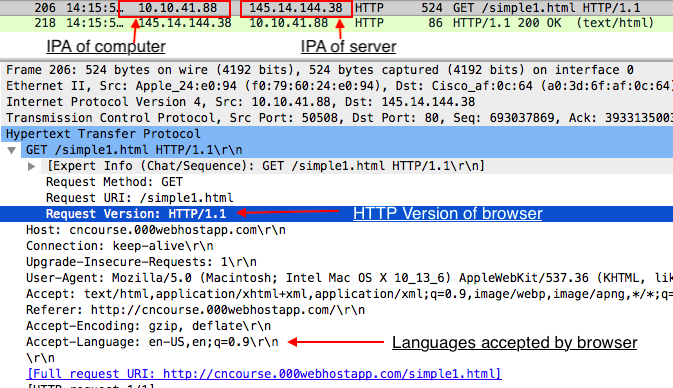
\includegraphics[height = 200pt, keepaspectratio]{Snapshots/q1/simple1/1_1.png}
\end{figure}
As highlighted, version \textbf{1.1} is used by both browser and server. 
\subsection{Languages accepted by the browser:}
As shown above, \textbf{English} language is accepted. 
\subsection{IPA of computer and \textit{cncourse} web server:}
IPA of computer is $10.10.41.88$ and that of server is $145.14.144.38$. 
\subsection{Status code returned from server to the browser: \textit{200}}
\begin{figure}[H]
	\vspace{0pt}
	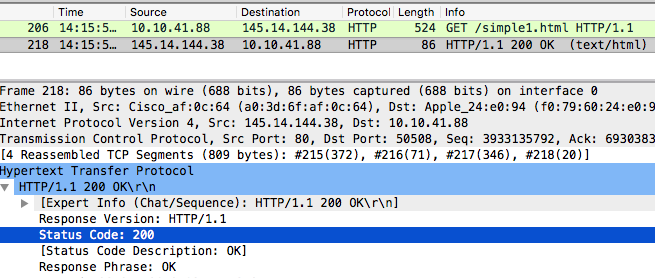
\includegraphics[height = 100pt, keepaspectratio]{Snapshots/q1/simple1/1_4.png}
\end{figure}
\subsection{HTML file last modified at the server:}
There is no \textit{last-modified} header in the HTTP packet. 
\subsection{Bytes of content returned to the browser:}
\begin{figure}[H]
  	\vspace{0pt}
  	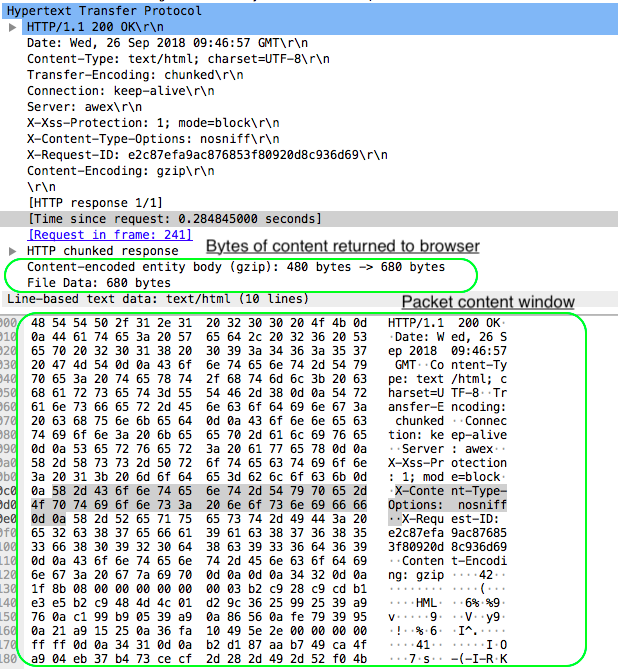
\includegraphics[height = 300pt, keepaspectratio]{Snapshots/q1/simple1/1_7.png}
\end{figure}
As highlighted, 480 bytes are returned to browser in \textit{gzip} format which is then uncompressed to 680 bytes by the browser.
\subsection{Headers not displayed in the packet-listing window:}
As seen in the packet content window, all the headers shown in the packet-listing window are only displayed, so there is NO additional header present.
\subsection{No. of request sent by browser and responded by server:}
\begin{figure}[H]
	\vspace{0pt}
	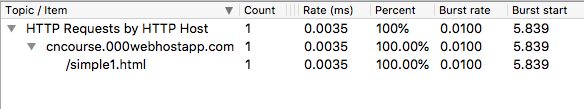
\includegraphics[height = 75pt, keepaspectratio]{Snapshots/q1/simple1/1_8.png}
\end{figure}
There is one request sent by the browser to the \textit{simple1.html} file on the server, and same is responded back by the server. 
\subsection{HTTP traffic flow graph showing the packet exchanges between the client and the server:}
The \textit{HTTP traffic flow} graph is obtained from the \textbf{Statistics - Flow Graph} option and then checking the option \textit{Limit to display filter} as the filter chosen is HTTP.
\begin{figure}[H]
	\vspace{0pt}
	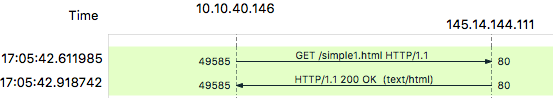
\includegraphics[height = 75pt, keepaspectratio]{Snapshots/q1/simple1/1_9.png}
\end{figure}
\subsection{File \textit{simple2.html}:}
\textbf{Last modified} information is not available for the \textit{html} file but for the \textit{GIF} image loaded along with this html, it is displayed below.
\begin{figure}[H]
	\vspace{0pt}
	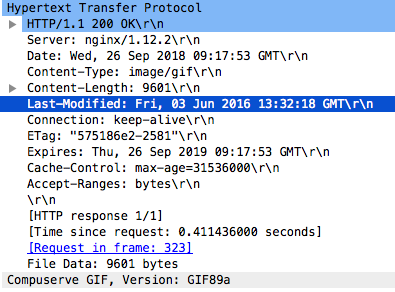
\includegraphics[height = 150pt, keepaspectratio]{Snapshots/q1/simple2/1_2_5.png}
\end{figure}
\textbf{Bytes of content} returned for the HTML file is $572$ bytes. That for the GIF is 9601 bytes.
\begin{figure}[H]
	\vspace{0pt}
	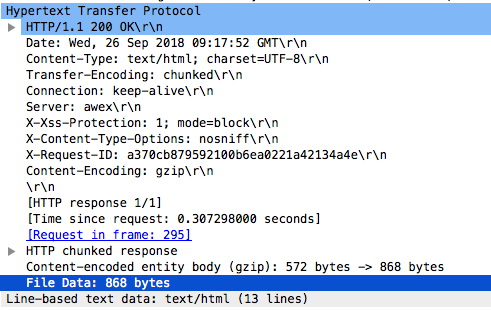
\includegraphics[height = 150pt, keepaspectratio]{Snapshots/q1/simple2/1_2_6.png}
\end{figure}
\textbf{No. of requests sent by the browser and responded by the server} are both $2$, as shown below. 
\begin{figure}[H]
	\vspace{0pt}
	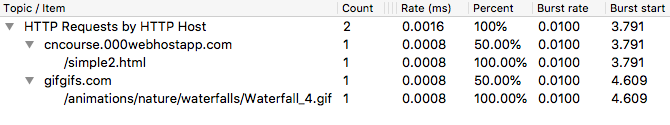
\includegraphics[height = 70pt, keepaspectratio]{Snapshots/q1/simple2/1_2_8.png}
\end{figure}
\textbf{HTTP Traffic Flow graph:}
\begin{figure}[H]
	\vspace{0pt}
	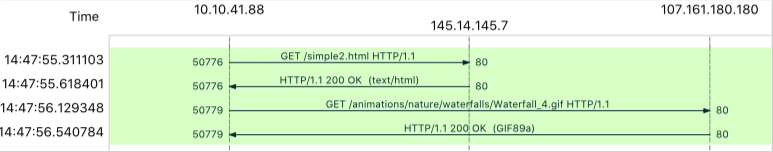
\includegraphics[height = 80pt, keepaspectratio]{Snapshots/q1/simple2/1_2_9.png}
\end{figure}
\subsection{File \textit{simple3.html}:}
\textbf{Last modified} information is not available for the \textit{simple3.html} file.
\begin{figure}[H]
	\vspace{0pt}
	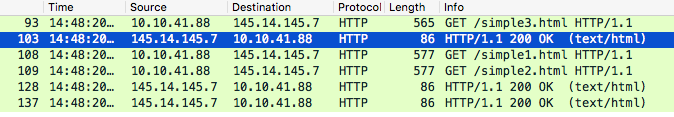
\includegraphics[height = 70pt, keepaspectratio]{Snapshots/q1/simple3/1_III.png}
\end{figure}
\textbf{Bytes of content} returned for the HTML file is $138$ bytes for \textit{simple3.html}. It also loads \textit{simple1.html} and \textit{simple2.html} whose sizes were mentioned earlier. 
\begin{figure}[H]
	\vspace{0pt}
	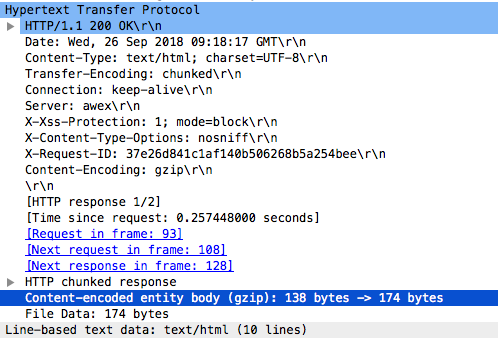
\includegraphics[height = 150pt, keepaspectratio]{Snapshots/q1/simple3/1_3_6.png}
\end{figure}
\textbf{No. of requests sent by the browser and responded by the server} are both $3$, as shown below. 
\begin{figure}[H]
	\vspace{0pt}
	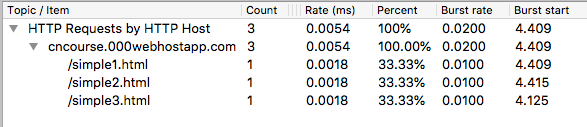
\includegraphics[height = 70pt, keepaspectratio]{Snapshots/q1/simple3/1_3_8.png}
\end{figure}
\textbf{HTTP Traffic Flow graph:}
\begin{figure}[H]
	\vspace{0pt}
	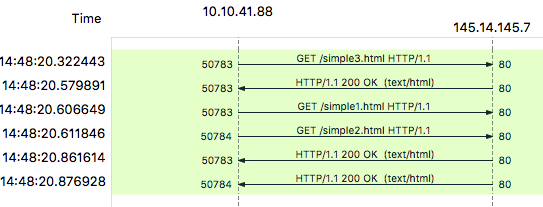
\includegraphics[height = 130pt, keepaspectratio]{Snapshots/q1/simple3/1_3_9.png}
\end{figure}
\subsection{File \textit{simple4.html}:}
\begin{figure}[H]
	\vspace{0pt}
	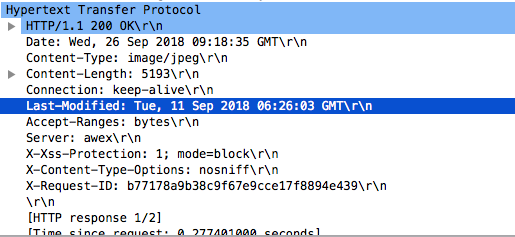
\includegraphics[height = 110pt, keepaspectratio]{Snapshots/q1/simple4/1_4_5.png}
\end{figure}
\textbf{Last modified} information is not available for the \textit{simple4.html} file but its present for the JPEG image files loaded from another server, as shown above for one such image. \\ 
\textbf{Bytes of content} returned for the HTML file is $535$ bytes for \textit{simple4.html}. It also loads 10 other image files.
\begin{figure}[H]
	\vspace{0pt}
	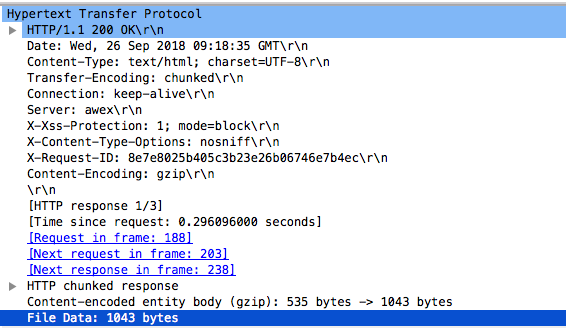
\includegraphics[height = 160pt, keepaspectratio]{Snapshots/q1/simple4/1_4_6.png}
\end{figure}
\textbf{No. of requests sent by the browser and responded by the server} are both $11$, as shown below. \\
\begin{figure}[H]
	\vspace{0pt}
	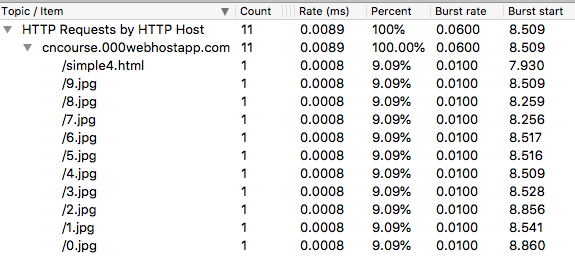
\includegraphics[height = 150pt, keepaspectratio]{Snapshots/q1/simple4/1_4_8.png}
\end{figure}
\textbf{HTTP Traffic Flow graph:}
\begin{figure}[H]
	\vspace{0pt}
	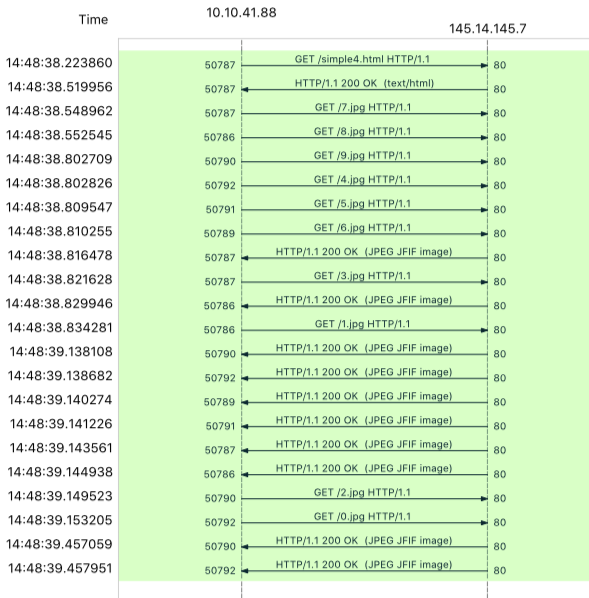
\includegraphics[height = 300pt, keepaspectratio]{Snapshots/q1/simple4/1_4_9.png}
\end{figure}
\subsubsection{Whether images downloaded serially or parallely:}
The image downloads occurred \textit{parallelly}. We can say so since in the above traffic flow graph, its clearly visible that the requests for the images 7.jpg, 8.jpg, 9.jpg, ..., all were made in a single go without waiting for response of either of the image to be available. The first response is available after 6 images were already requested. 
\subsection{Time required to access the pdf file:}

\subsection{Table for time required to access each of the files:}
-
%%%%%%%%%%%%%%%%%%%%%%%%%%%%%%%%%%%%%%%%%%%%%%%%


\section{The HTTP CONDITIONAL GET/Response Interaction:}
\subsection{First HTTP GET request from the browser to the server:}

\subsection{Contents of the server response:}

\subsection{Second HTTP GET request from the browser to the server: }

\subsection{HTTP status code and phrase returned from the server in response to 2nd HTTP GET:}
-
%%%%%%%%%%%%%%%%%%%%%%%%%%%%%%%%%%%%%%%%%%%%%%%%


\section{Retrieving Long Documents:}
\subsection{HTTP GET request messages sent by the browser:}

\subsection{Packet no in trace containing the status code and phrase associated with the response to the HTTP GET request:}

\subsection{Status code and phrase in the response:}

\subsection{No. of data-containing TCP segments needed to carry the single HTTP response and the text of the file:}
-
%%%%%%%%%%%%%%%%%%%%%%%%%%%%%%%%%%%%%%%%%%%%%%%%


\section{HTML Documents with CGI Script:}
\subsection{Method used in the HTTP message:}

\subsection{No. of HTTP request messages sent by the browser:}

\subsection{IPA to which the requests are sent:}
-
%%%%%%%%%%%%%%%%%%%%%%%%%%%%%%%%%%%%%%%%%%%%%%%%


\section{HTTP Authentication:}
\subsection{Server response to the initial HTTP GET message:}

\subsection{New field included in HTTP GET message when browser sends request for 2nd time:}

\subsection{Content of packet in wireshark where password is displayed:}
-
%%%%%%%%%%%%%%%%%%%%%%%%%%%%%%%%%%%%%%%%%%%%%%%%

\end{document}